\section{Results}
\label{sec:results}

In this section we describe the reaching performance obtained with 
the reaching controller described in the previous section. Within this context,
it is important to note that a formal definition of the performance 
index is a nontrivial task. 

If we were to consider a robot which operates in an highly structured
environment, the definition of the performance index would have been much easier. 
Specifically, for an industrial robot, the reaching task can be identified 
with the problem of positioning the hand accurately with respect to a world 
reference frame\footnote{Typical industrial robots do not use vision. Their 
grasping movement is the result of 3-D positioning the gripper exactly in the 
position where they know the object to be grasped will be positioned. The problem
of positioning the object is then left to the user.}. In this case, the reaching 
precision can be measured in terms of the distance between the desired and 
actual position of the hand in the world reference frame.
 
In our case, a similar performance index definition cannot be applied. James has not 
been designed to operate in an industrial scenario. Moreover, in our context, the definition of a reference 
frame fixed with respect to the external world does not play the same crucial 
role played in the industrial framework. In our mind, it is more important to 
precisely locate the hand with respect to the object than to precisely locate 
the hand in the external world frame. Therefore, our reaching performance index 
should measure the Cartesian distance between the object to be grasped and the final 
position of the hand. However, measuring this distance is not an easy task. In this section
we approximate the real distance with the (stereo) \emph{image plane distance}. Practically speaking, suppose the 
robot sees a target $\utarget$ to be grasped. Following our strategy, in order to reach the 
target we need to fixate it, i.e. $\utarget = 0$. Using the available sensor (i.e. vision) the best we can do to precisely reach the target is moving the hand to the fixation point, i.e. $
{\uhand} \longrightarrow 0$. Clearly, the image plane distance $\| \uhand - \utarget \|$ can be used as a rough estimate of the reaching precision, i.e. of the Cartesian distance between the target to be reached and the position of the hand. Specifically, assuming infinite resolution of the camera sensor, if $\| \uhand - \utarget\| = 0$ then the hand has exactly reached the target. In a more realistic case, when the image plane distance is null, we can only guarantee that the Cartesian target-hand distance is upper bounded by a quantity which depends only on the camera intrinsic parameters\footnote{
Computing this upper bound is out of the scope of this paper.}. 

\subsection{Open Loop}
The first attempt to reach the target consists in using (\ref{Eq:reaching2})
to choose the arm configuration $\q_{arm}$ which brings the hand to the center 
of the image planes. Clearly, if the forward 
kinematic function (\ref{Eq:forward}) were perfectly represented and if the target were reachable, we would have $\mathbf x_{hand} =  \mathbf x_{target}$, which implies that the target-hand Cartesian distance 
 is null (see Section \ref{sec:reaching} for details). Therefore, in this ideal case, the open loop 
 strategy already results in $\| \uhand - \utarget \| = 0$. In practice, the model 
 (\ref{Eq:forward}) cannot exactly represent the system kinematic\footnote{Part of the representational 
 errors are related to the way we have chosen the represent the kinematic function, in this case the
 so called Receptive Field Weighted Regression model. Part are due to the mechanical plays of the
 kinematic structure.}. Therefore, even tough we can find $\q_{arm}$ such that $\mathbf x_{hand}=
 \hat f_{arm}(\mathbf q_{arm})$ it is not guaranteed that after the movement execution 
 $\| \uhand - \utarget \| = 0$. Figure \ref{Fig:ImagePlaneOpenLoopErrors}
 shows the image plane errors after the execution of the open loop movement. The plot has been obtained
 by fixating a target and performing a series of open loop movements. Each open loop
 movement was different because (\ref{Eq:reaching2}) was solved 
 by choosing a different value $q_{20}$. Let us denote the open loop movements $\q_{arm}^1$, $\dots$, 
 $\q_{arm}^K$ such that:
 
 \begin{multline} \label{Eq:OpenLoopMovements}
 \q_{arm}^k = \arg \min_{\mathbf q_{arm}}
  \left[
  \left\| \hat f_{arm}(\mathbf q_{arm}) - \mathbf x_{target}\right\|^2 \right. \\ + \left. \left(q_{arm,2}-q_{20}^k\right)^2
  \right].
 \end{multline}
 
 The above minimization is such that $\hat f_{arm}(\mathbf q_{arm}^k) = \mathbf x_{target}$. Ideally, in absence
 of modeling errors we would have $ \mathbf x_{hand} = \mathbf x_{target}$ since $\mathbf x_{hand} = f_{arm}(\mathbf q_{arm}^k)$. In practice we have $\mathbf x_{hand} \simeq \hat f_{arm}(\mathbf q_{arm})$ 
 so that we can only achieve an approximate reaching $ \mathbf x_{hand} \simeq \mathbf x_{target}$ 
 which reflects into small image plane errors $\| \uhand - \utarget\| \simeq 0$. Different choices 
 of the free variables $q_{20}^1$, $\dots$, $q_{20}^K$ lead to different image plane errors as shown 
 in Figure \ref{Fig:ImagePlaneOpenLoopErrors}.



\begin{figure}
  % Requires \usepackage{graphicx}
  \begin{center}
	\begin{tabular}{ccc}
	  \parbox{30mm}{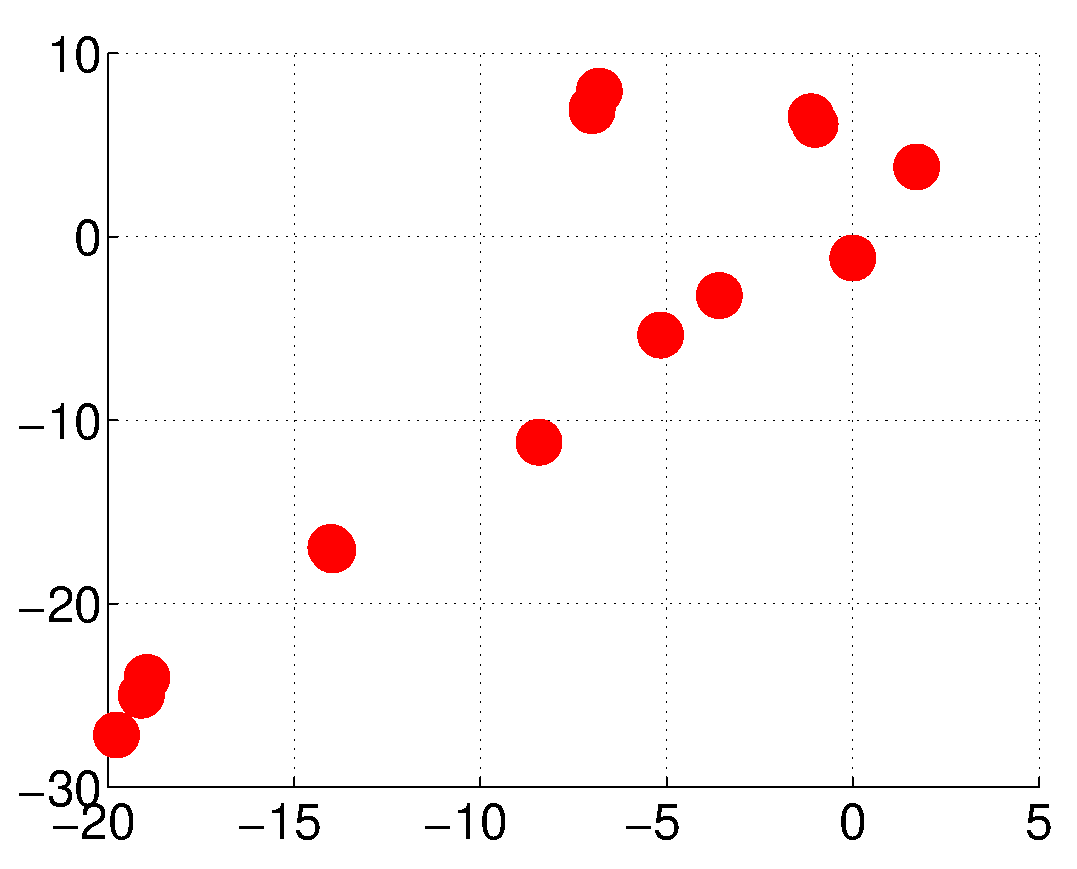
\includegraphics[width=30mm]{Figure/LeftEyeOpenLoop.eps}}  & \hspace{0.1cm} &
	  \parbox{30mm}{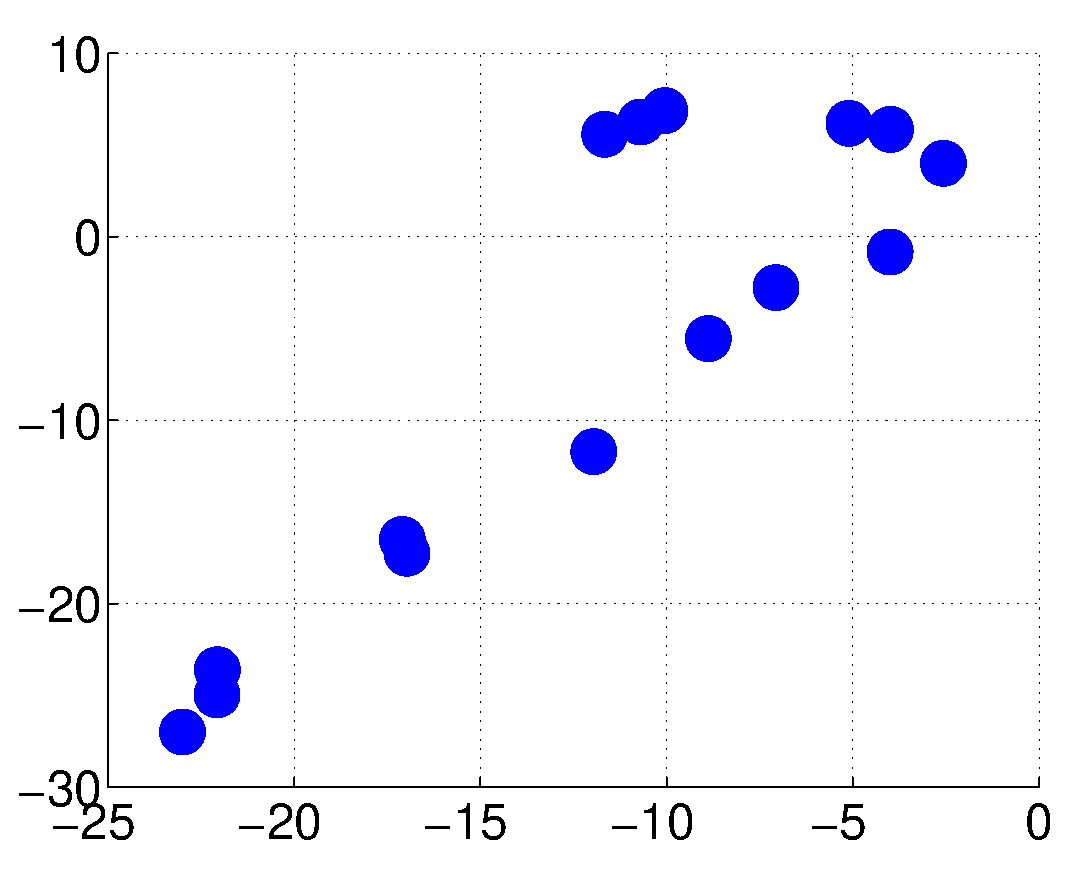
\includegraphics[width=30mm]{Figure/RightEyeOpenLoop.eps}}
	  \\
	  \parbox{30mm}{\centering Left eye } & \hspace{0.1cm} & \parbox{30mm}{\centering Right eye }
	  %	  \end{t\\
	  %	Top view & & Lateral view
  \end{tabular}
\end{center}
\caption{Open loop image plane errors $\uhand$ for different
choices of the redundant variable $q_{20}$. For both pictures, on the horizontal axis 
we have $u_r$ and $u_l$ while on the vertical axis we have $v_r$ and $v_l$ (always in pixels).
In this specific case the target is in the middle of the two image planes 
$[u_{r, target}, v_{r, target}] =[0,0]$ and $[u_{l, target}, v_{l, target}]=[0,0]$.
The hand position in the image plane is instead represented 
by the small circles.  Each circle corresponds to the hand position 
after a different open loop movement, i.e. a different value of $q_{20}$.
}\label{Fig:ImagePlaneOpenLoopErrors}
  \end{figure}

\subsection{Closed Loop}

As we described in Section \ref{Eq:ClosedLoop} the residual image plane errors 
due to imperfections in the forward kinematic model can be reduced by a visual closed loop
control strategy. This control strategy moves the arm so as to progressively 
drive the hand position in the image planes ($\mathbf x_{hand}$) to zero. Of course this is guaranteed 
only if the  Jacobian matrix has been learned in a sufficient accuracy. Figures 
\ref{Fig:ImagePlaneClosedLoopErrors}, \ref{Fig:TimeResponseClosedLoopErrors},  \ref{Fig:TimeResponseOpenClosedLoop} and \ref{Fig:TimeResponseOpenClosedLoopErrors} 
show how the hand is actually driven to the 
exact image center in both the image planes. Moreover, it is important to notice the
approximative linearity of the path followed by the hand. This linearity denotes 
a good accuracy of the learned Jacobian.

\begin{figure}
  % Requires \usepackage{graphicx}
  \begin{center}
	\begin{tabular}{ccc}
	  \parbox{30mm}{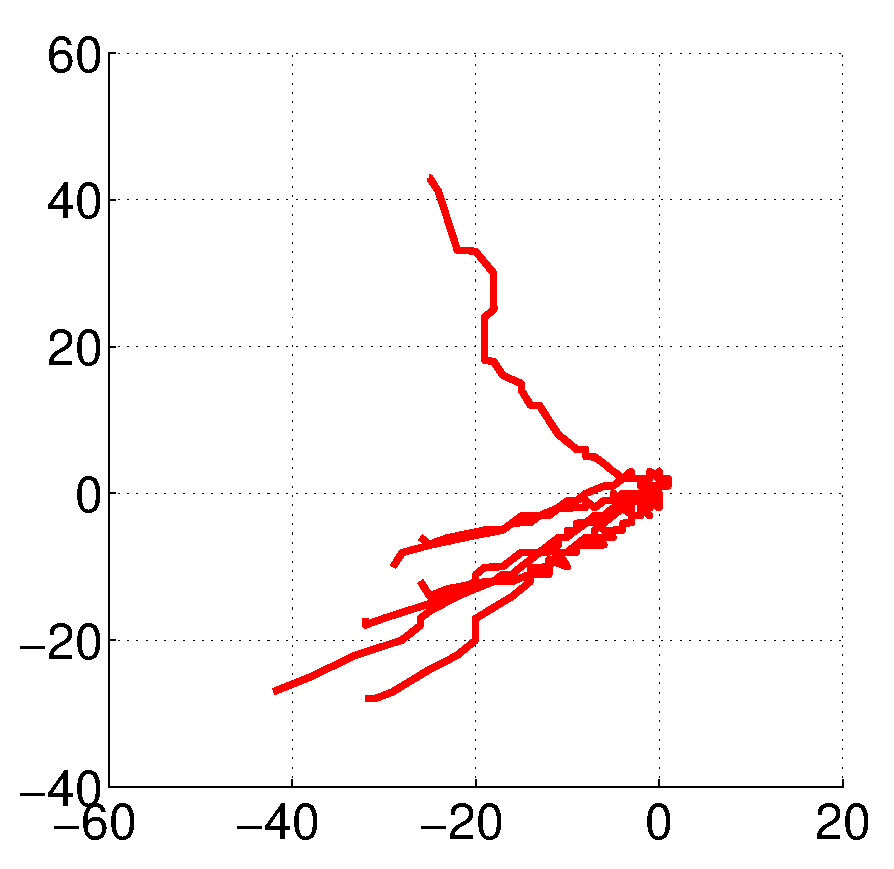
\includegraphics[width=30mm]{Figure/LeftEyeClosedLoop.eps}}  & \hspace{.1cm} &
	  \parbox{30mm}{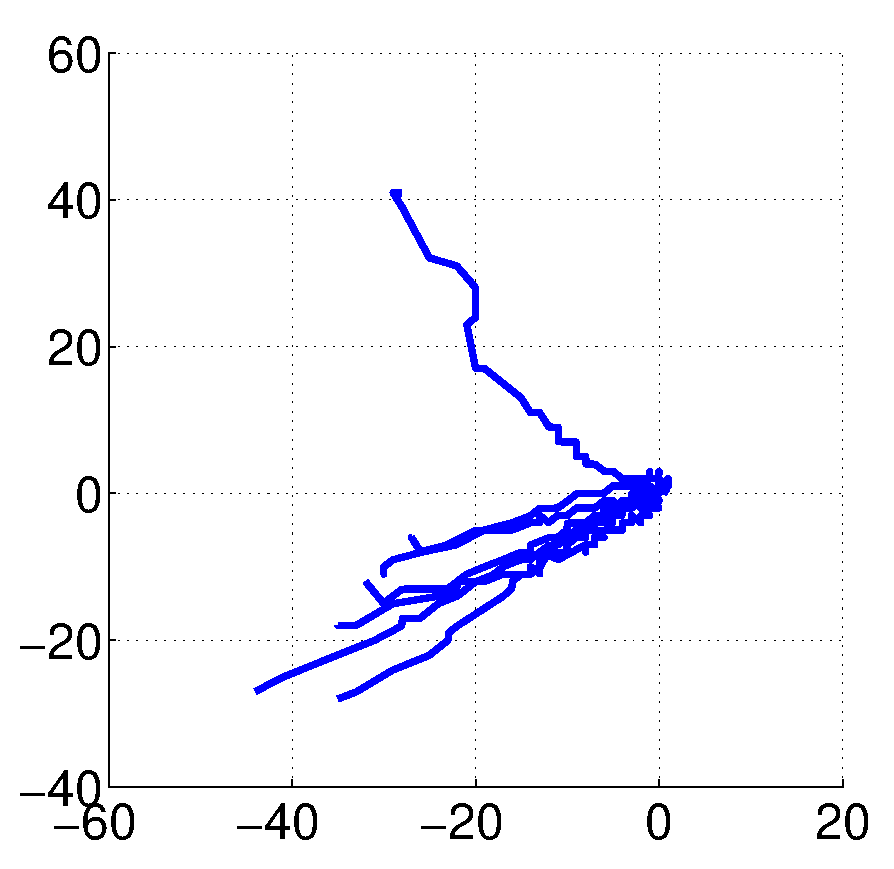
\includegraphics[width=30mm]{Figure/RightEyeClosedLoop.eps}}
	  \\
	  \parbox{30mm}{\centering Left eye } & \hspace{0.1cm} & \parbox{30mm}{\centering Right eye }
	  %	  \end{t\\
	  %	Top view & & Lateral view
  \end{tabular}
\end{center}
\caption{Traces of different closed loop control actions. Each trace correspond to a different Cartesian position of the target to be reached (which 
is always at the center of the image planes). The traces start exactly after the execution of the open loop movement, so that the initial position corresponds to the initial open loop error. Notice that all the traces end up in the image center (both left and right image planes) thus indicating that the visual errors are completely eliminated by the closed loop controller.}\label{Fig:ImagePlaneClosedLoopErrors}
  \end{figure}

\begin{figure}
  % Requires \usepackage{graphicx}
  \begin{center}
	\begin{tabular}{ccc}
	  \parbox{30mm}{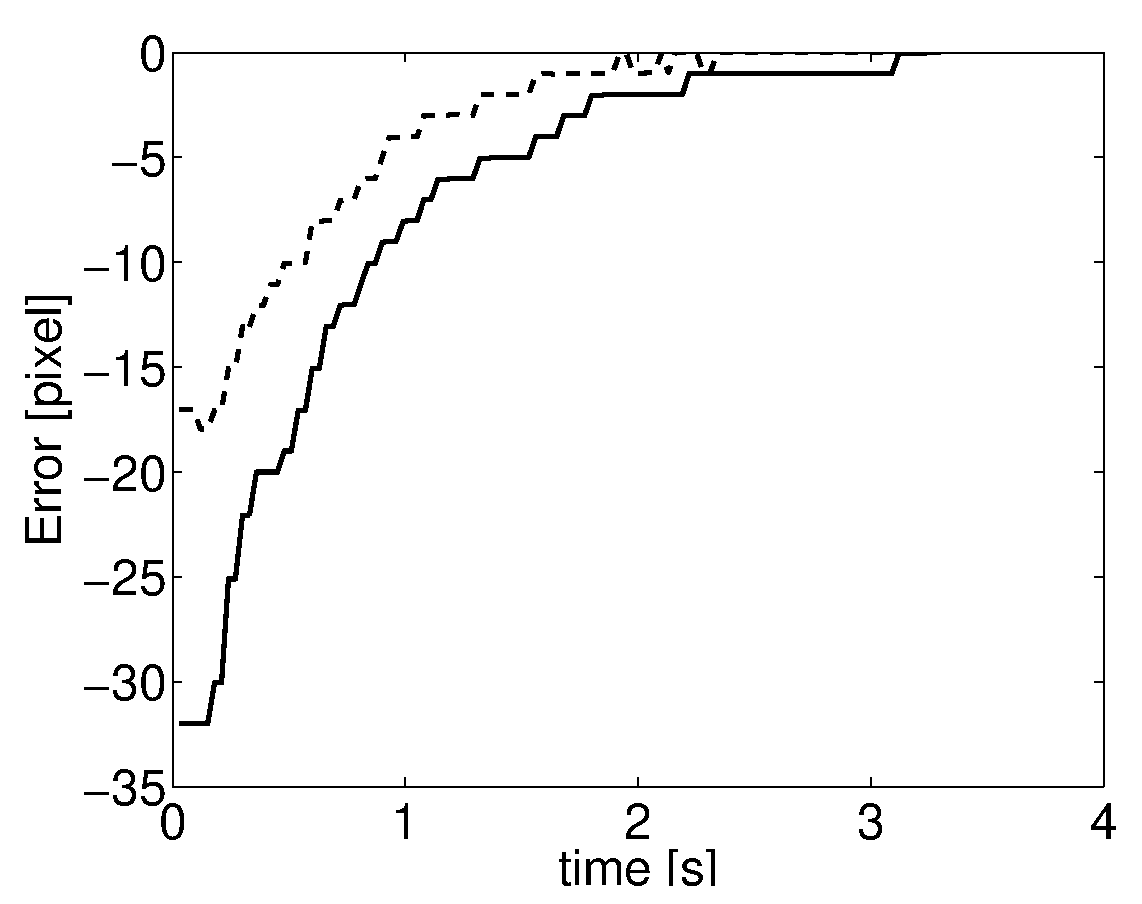
\includegraphics[width=30mm]{Figure/TimeReponseLeftClosedLoop.eps}}  & \hspace{.1cm} &
	  \parbox{30mm}{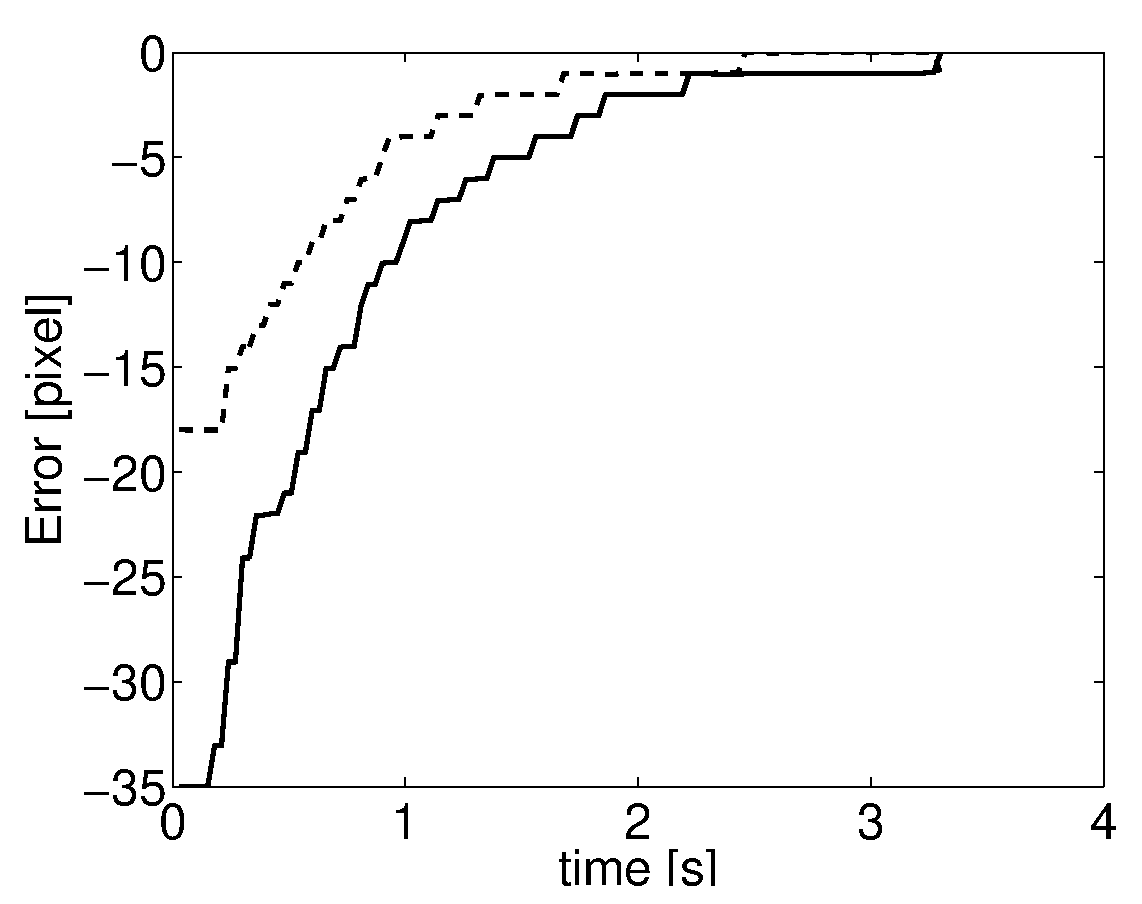
\includegraphics[width=30mm]{Figure/TimeReponseRightClosedLoop.eps}}
	  \\
	  \parbox{30mm}{\centering Left eye } & \hspace{0.1cm} & \parbox{30mm}{\centering Right eye }
	  %	  \end{t\\
	  %	Top view & & Lateral view
  \end{tabular}
\end{center}
\caption{Time response of the closed loop controller. The solid lines corresponds to the hand horizontal position in the left ($u_l$) and right ($u_r$) image planes. The dashed lines correspond to the vertical position, $v_l$ and $v_r$. Clearly, the hand is driven to the image center with a null steady state error. Even if velocity was not our primarily concern, the time response is reasonably fast (an error of thirty pixels is eliminated in about 
three seconds). }\label{Fig:TimeResponseClosedLoopErrors}
  \end{figure}


\begin{figure}
  % Requires \usepackage{graphicx}
  \begin{center}
	\begin{tabular}{ccc}
	  \parbox{30mm}{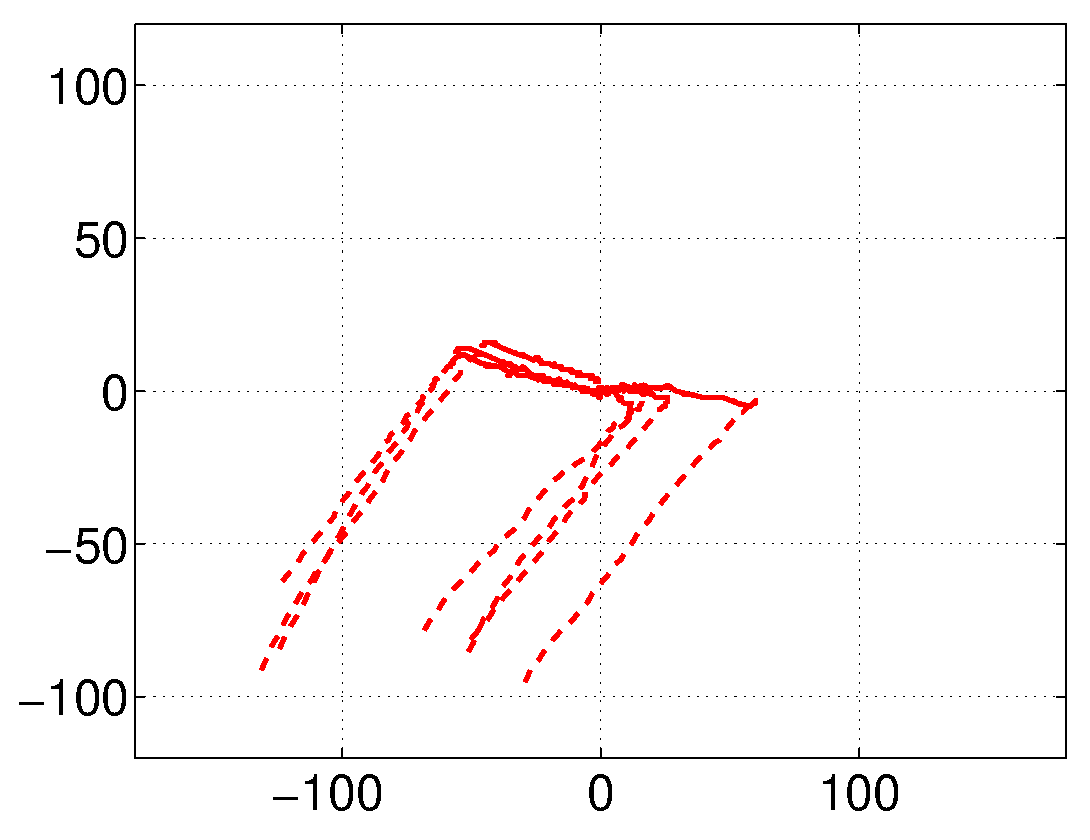
\includegraphics[width=30mm]{Figure/LeftEyeOpenClosedLoop.eps}}  & \hspace{.1cm} &
	  \parbox{30mm}{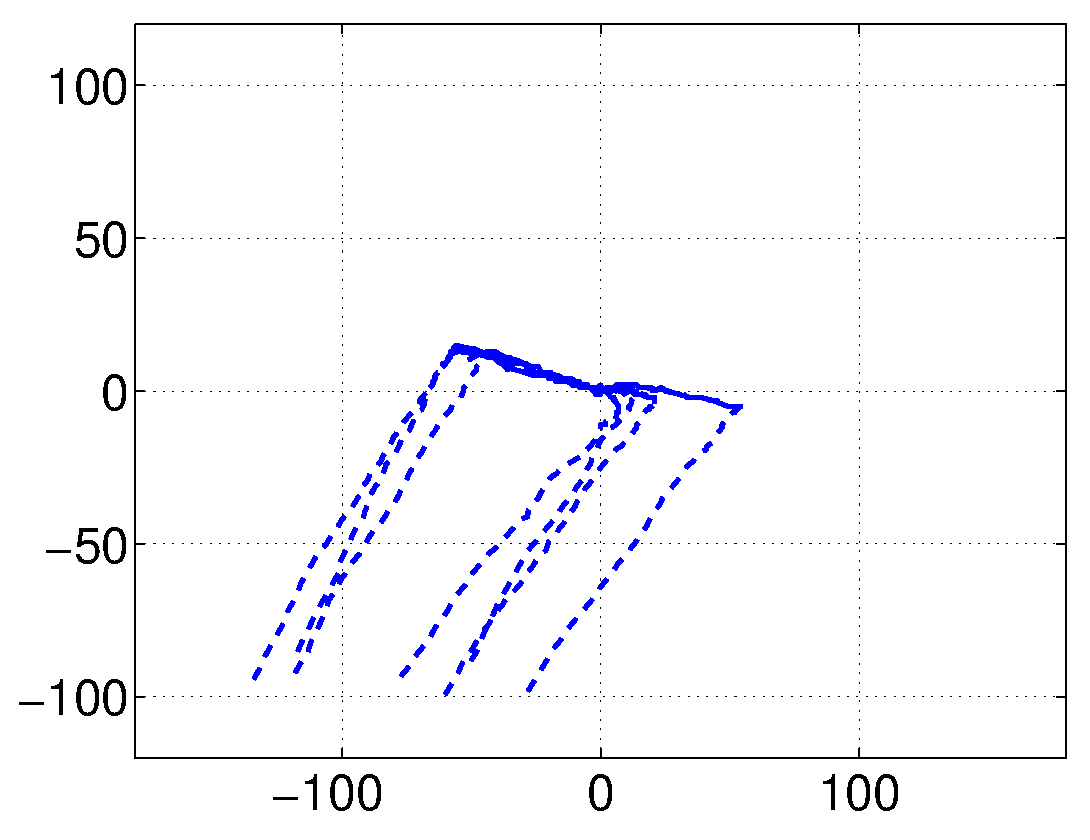
\includegraphics[width=30mm]{Figure/RightEyeOpenClosedLoop.eps}}
	  \\
	  \parbox{30mm}{\centering Left eye } & \hspace{.1cm} & \parbox{30mm}{\centering Right eye }
	  %	  \end{t\\
	  %	Top view & & Lateral view
  \end{tabular}
\end{center}
\caption{Movement of the hand on the image planes (320$\times$240)
during the execution of different reaching actions. For both pictures, 
on the horizontal axis 
we have $u_r$ and $u_l$ while on the vertical axis we have $v_r$ and $v_l$ (always in pixels).
The traces correspond to the hand position during the movement. The solid line is the hand movement
during the closed loop phase. The dashed trace is instead the hand movement during the open loop 
phase. Clearly the open loop movement drives the hand to the target (the image centers) with a 
relatively small error. The closed loop phase reduces this error to zero.}\label{Fig:TimeResponseOpenClosedLoopErrors}
  \end{figure}
  
  \begin{figure}
  % Requires \usepackage{graphicx}
  \begin{center}
	\begin{tabular}{ccc}
	  \parbox{30mm}{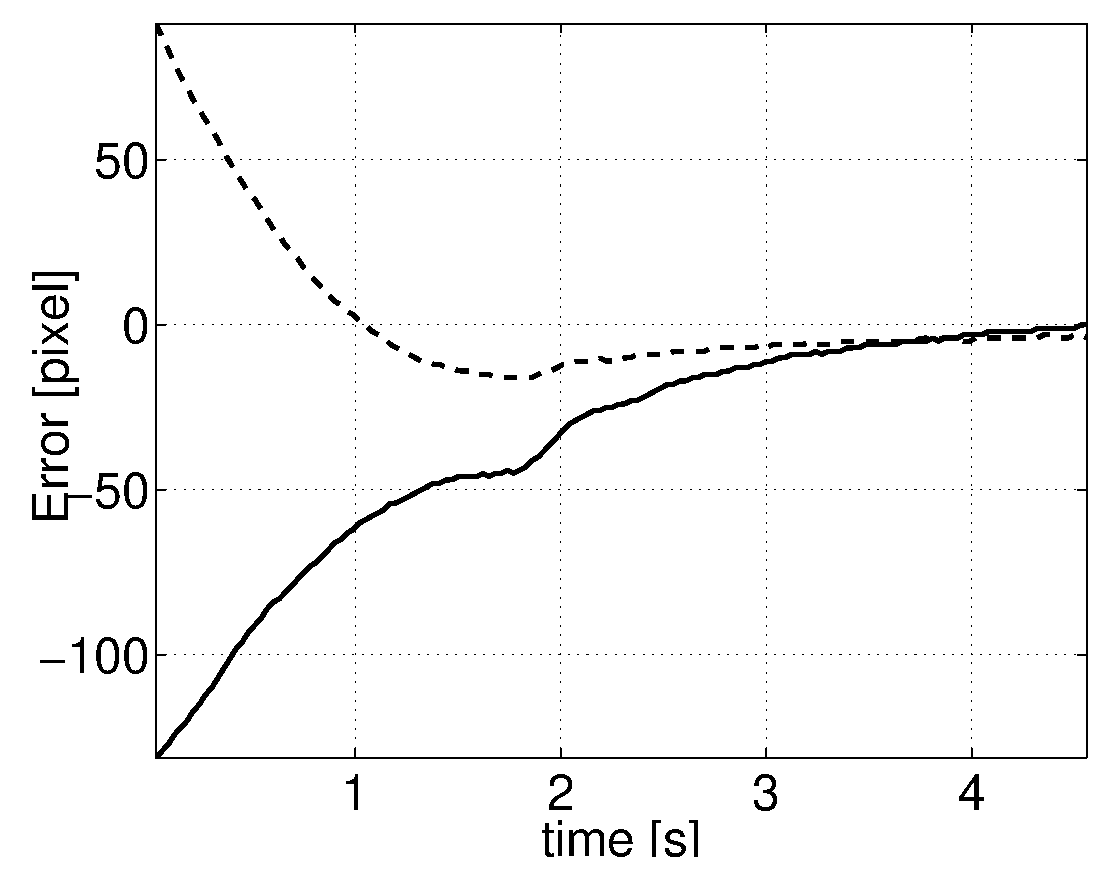
\includegraphics[width=30mm]{Figure/LeftEyeOpenClosedLoopTimeResponse.eps}}  & \hspace{.1cm} &
	  \parbox{30mm}{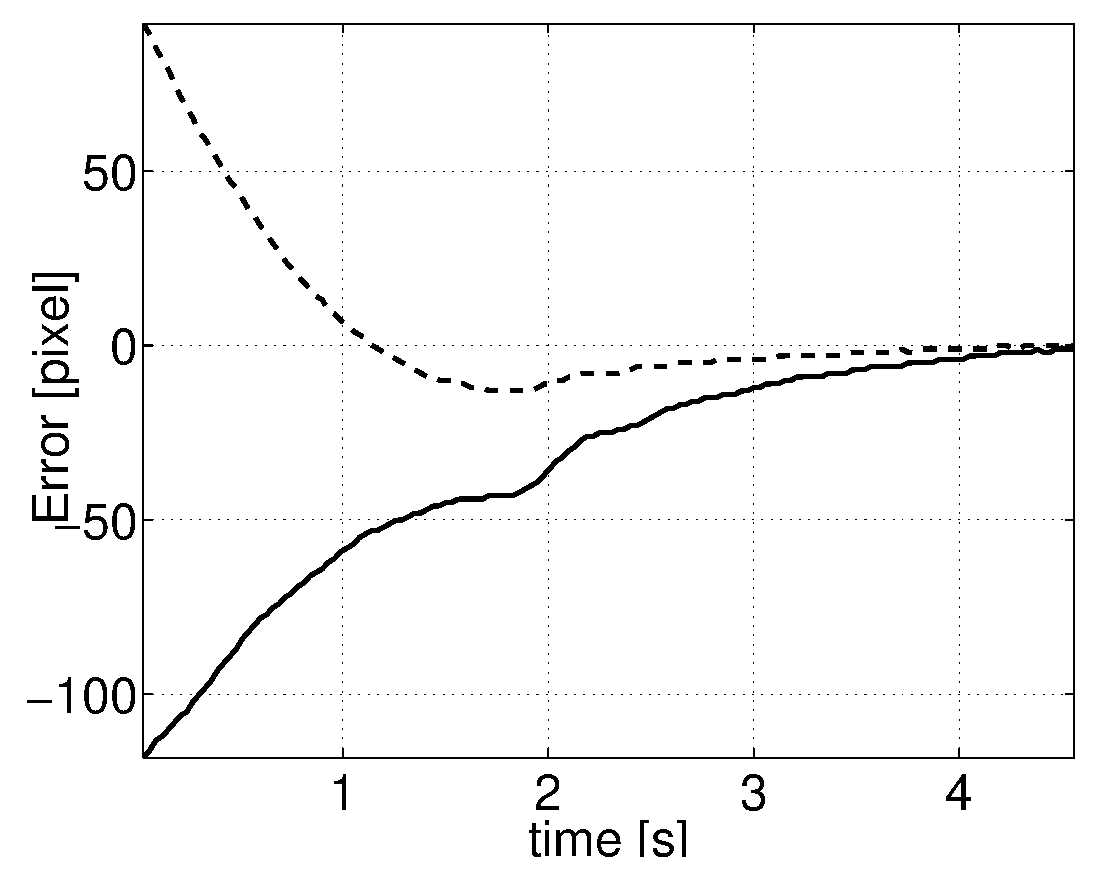
\includegraphics[width=30mm]{Figure/RightEyeOpenClosedLoopTimeResponse.eps}}
	  \\
	  \parbox{30mm}{\centering Left eye } & \hspace{.1cm} & \parbox{50mm}{\centering Right eye }
	  %	  \end{t\\
	  %	Top view & & Lateral view
  \end{tabular}
\end{center}
\caption{Time response of the closed loop and open loop strategy. The solid lines correspond to the hand horizontal position in the left ($u_l$) and right ($u_r$) image planes. The dashed lines correspond to the vertical position, $v_l$ and $v_r$. Remarkably, the open loop phase is faster but does not drive the hand exactly on the target. The closed loop is slower but more accurate.}\label{Fig:TimeResponseOpenClosedLoop}
  \end{figure}